\chapter{Instrukcja uruchomienia}

\section{Przed rozpoczęciem}
Przed uruchomieniem projektu należy upewnić się, że posiadane są wymagane składniki:

\begin{itemize}
    \item \textbf{Program Docker} - Jeżeli Docker nie jest zainstalowany na komputerze, należy go pobrać i zainstalować zgodnie z instrukcją na oficjalnej stronie: \href{https://docs.docker.com/desktop/}{https://docs.docker.com/desktop/}. 
    \item \textbf{Aplikacja CN-Project} - Należy upewnić się, że projekt znajduje się na używanej maszynie i nic nie blokuje dostępu do niego. Jeżeli projekt nie znajduje się na lokalnym sprzęcie, należy go pobrać przy użyciu programu Git i komendy: 
    \begin{quote} 
        \texttt{git clone https://github.com/KarolZygadlo/CN-Project.git} 
    \end{quote} 
\end{itemize}

\section{Uruchomienie projektu}
Aby uruchomić projekt „CN-Project” na swoim komputerze, należy wykonać następujące kroki:

\begin{enumerate} 
    \item Uruchomić program Docker Desktop na swoim systemie operacyjnym. 
    \item W konsoli systemu operacyjnego przejść do folderu, w którym znajduje się projekt (folder nazywa się \texttt{CN-Project}). 
    \item Projekt zostanie uruchomiony po wpisaniu i zatwierdzeniu poniższej komendy. Uruchomi ona kontenery w tle: 
    \begin{quote} 
        \texttt{docker compose up -d} 
    \end{quote} 
    \textit{Flagi:} 
    \begin{itemize} 
        \item \texttt{-d} - oznacza uruchomienie kontenerów w trybie odłączonym (w tle), co pozwala na dalsze korzystanie z terminala. 
    \end{itemize} Jeżeli chcemy widzieć logi kontenerów na bieżąco, należy użyć tej samej komendy, ale bez flagi \texttt{-d}: 
    \begin{quote} 
        \texttt{docker compose up}
    \end{quote} 
    \textit{Uwaga: Proces uruchamiania może potrwać kilka minut, szczególnie przy pierwszym uruchomieniu, ponieważ Docker pobiera wszystkie niezbędne obrazy i zależności.} 
    \item Po pobraniu i uruchomieniu projektu, aplikacja webowa będzie dostępna pod adresem \texttt{localhost}. Należy wpisać ten adres w przeglądarkę, aby wyświetlić stronę główną aplikacji. 
    \item Aby wyłączyć kontenery, należy wpisać w konsolę komendę: 
    \begin{quote} 
        \texttt{docker compose down} 
    \end{quote} Ta komenda zatrzyma wszystkie uruchomione kontenery. 
\end{enumerate}

\section{Wejście do kontenera}
W przypadku, gdy konieczne jest skorzystanie z narzędzi wewnątrz kontenera, najlepszym sposobem jest uruchomienie powłoki kontenera z poziomu maszyny lokalnej.

Poniższe kroki opisują sposób uruchomienia powłoki kontenera PHP.

\begin{enumerate} 
    \item Kontener musi być włączony. Można to sprawdzić przy pomocy komendy: 
    \begin{quote} 
        \texttt{docker ps} 
    \end{quote} Komenda ta pokazuje tylko aktualnie włączone kontenery.
    
    Poniżej przykład wyniku wywołania komendy \texttt{docker ps}:
    \begin{figure}[h]
        \centering
        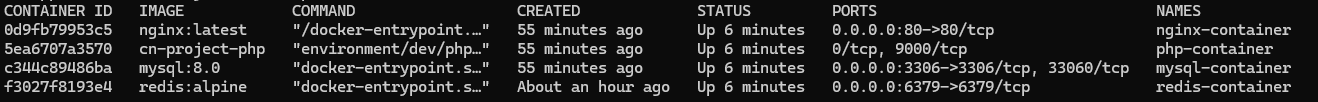
\includegraphics[width=\textwidth]{images/docker_ps.png}
    \end{figure}

    \textit{Ostatnia kolumna wskazuje nazwy kontenerów — nazwa kontenera będzie używana do odwoływania się do niego.}

    \item Korzystając z nazwy kontenera (np. \texttt{php-container}), można uruchomić powłokę kontenera PHP przy użyciu komendy:
    \begin{quote}
        \texttt{docker exec -it php-container sh}
    \end{quote}
    
    \textit{Elementy komendy:}
    \begin{itemize}
        \item \verb|docker exec -flagi [nazwa kontenera] [polecenia]| - wykonuje wybrane polecenie w wybranym konenerze. 
        \item \verb|-it| - Flaga \verb|-i| oznacza „interaktywny” tryb, co pozwala na komunikację z kontenerem, a \verb|-t| tworzy terminal, który umożliwia korzystanie z powłoki w trybie tekstowym.
        \item \verb|sh| - uruchamia powłokę systemu operacyjnego w kontenerze. Można używać innych powłok, takich jak \verb|bash|, jeżeli są dostępne w kontenerze.
    \end{itemize}
    
    Po zatwierdzeniu komendy użytkownik znajduje się wewnątrz kontenera i ma dostęp do wszystkich plików i programów, które się w nim znajdują.
\end{enumerate}